\documentclass[runningheads]{llncs}
%
\usepackage{graphicx}
\usepackage{algpseudocode,algorithm}
\usepackage{hyperref}
\usepackage{listings}
\usepackage{xcolor}
\usepackage{xstring}
\usepackage[nointegrals]{wasysym}
\usepackage{MnSymbol}
\usepackage{booktabs} % For formal tables
\graphicspath{ {../images/} }

\definecolor{NavyBlue}{HTML}{000080}
\definecolor{Magenta}{HTML}{FF00FF}
\definecolor{Orange}{HTML}{FFA500}
\definecolor{CornflowerBlue}{HTML}{6495ED}
\definecolor{YellowGreen}{HTML}{9ACD32}
\definecolor{Gray}{HTML}{BEBEBE}
\definecolor{Yellow}{HTML}{FFFF00}
\definecolor{GreenYellow}{HTML}{ADFF2F}
\definecolor{ForestGreen}{HTML}{228B22}
\definecolor{Lavender}{HTML}{FFC0CB}
\definecolor{SkyBlue}{HTML}{87CEEB}
\definecolor{NavyBlue}{HTML}{000080}
\definecolor{Goldenrod}{HTML}{DDF700}
\definecolor{VioletRed}{HTML}{D02090}
\definecolor{CornflowerBlue}{HTML}{6495ED}
\definecolor{LimeGreen}{HTML}{32CD32}


\begin{document}
\title{Event-driven multi-population optimization: mixing Swarm and
  Evolutionary strategies}
\titlerunning{Event-driven multi-population optimization}
\author{First Author\inst{1}\orcidID{0000-1111-2222-3333} \and
Second Author\inst{2,3}\orcidID{1111-2222-3333-4444} \and
Third Author\inst{3}\orcidID{2222--3333-4444-5555}}
%
\authorrunning{F. Author et al.}

\institute{Princeton University, Princeton NJ 08544, USA \and
Springer Heidelberg, Tiergartenstr. 17, 69121 Heidelberg, Germany
\email{lncs@springer.com}\\
\url{http://www.springer.com/gp/computer-science/lncs} \and
ABC Institute, Rupert-Karls-University Heidelberg, Heidelberg, Germany\\
\email{\{abc,lncs\}@uni-heidelberg.de}}
%
\maketitle              % typeset the header of the contribution
%
\begin{abstract}

Researchers in the field of nature-inspired optimization have recently
proposed multi-population asynchronous algorithms that distribute the
evolutionary process among heterogeneous search paradigms. These
algorithms execute the optimization strategy by reading streams of
messages containing solution populations from message queues. After
searching for a small number of iterations, new evolved populations
are generated and sent back to a queue. Current research suggests that
when we have many population-processing algorithms communicating in
parallel, parameters intensifying exploration or exploitation in each
population strike a dynamic that balances the two, exploring and
exploiting simultaneously, maintaining an overall diversity, and
improving the search.  In this work, we propose a simple reactive
migration, that is, population-generation and processing, method for
the asynchronous execution of multi-population, multi-strategy
algorithms that manages to achieve an improvement over homogeneous
configurations. We evaluate this method by comparing a heterogeneous
ensemble of multi-populations against a homogeneous solution
consisting of Genetic Algorithms (GAs) and Particle Swarm Optimization
(PSO) populations. We evaluate both solutions using five problems from
the noiseless BBOB testbed for the optimization of continuous
functions. Results show that compared with other asynchronous
homogeneous population-based algorithms, this method offers better
performance in terms of the number of evaluations needed to find a
solution and the number of instances where it found it.

\keywords{heterogeneous multi-population algorithms  \and genetic algorithms
 \and cloud-native systems.}
\end{abstract}
%
%
%
\section{Introduction}

The class of algorithms generically denominated nature-inspired
\cite{yang2014nature}, which  include evolutionary (EAs) and swarm
intelligence (SI) algorithms
\cite{back1996evolutionary,kennedy2006swarm}, have a lot of
characteristics in common.
Together with others like PBIL (Population Based Incremental Learning)
\cite{baluja1994population} and EDAs (Estimation of Distribution
algorithms) \cite{larranaga2001estimation} use (or generate, in the
case of EDA) a set of (initially) random candidate solutions to
produce a new set of candidates considering each candidate solutions'
fitness.

\begin{table}[h!tb]
    \caption{Equivalence of terms between particle swarm optimization
    and evolutionary algorithms. \label{tab:equivalence}}
\centering
\begin{tabular}{|c|c|}
  \hline
  PSO & EA \\ \hline
  Position vector & {\em genes} in a chromosome \\ \hline
  Move towards better & Selection  \\ \hline
  Random motion & Mutation \\ \hline
  Move towards centroid & Crossover \\ \hline
\end{tabular}
\end{table}
%
Additionally, EAs and PSOs share another characteristic, besides the fact that they
act on populations: they can use the same data structures to
represent  members of the population. Please check Table
\ref{tab:equivalence} for equivalence of terms between PSO and EAs;
additionally to the data structures used, there is a certain
equivalence in the operators, but they are different enough to perform
search in different ways. The fact that they use the same data
structures means that you can apply them in turns, or simply start
calling a ``chromosome'' a ``particle'' or the other way round,
without any conversion, and keep working with it with any of the
algorithms. We will get back to this a bit later.
They also face common challenges: Since all population members have to
be evaluated to obtain a fitness or score that will be used to select
them (or not), a disadvantage of this kind of algorithms is that they
can be computationally expensive: every candidate solution needs to be
evaluated, and the different strategies to efficiently explore the
search space might eventually lead to lots of evaluations.
This fact, together with the a priori ease of simultaneous evaluation
of different segments of the population, have spawned proposals of
some form of parallelization from the start
\cite{muhlenbein1988evolution} to decrease their execution time, at
least in the area of evolutionary algorithms. One of the first
parallelization methods was the island model, which led to an
increased performance
\cite{gorges1990explicit,grosso1985computer}. The idea was to divide
the population into smaller segments that interacted with each
other. Since then, other researchers have adopted the idea and found
additional advantages besides a reduced execution speed; these include
avoiding a premature convergence and maintaining the global
population's diversity \cite{li2015multi}. We are going to call these
kinds of methods, multi-population algorithms \cite{Ma2019}. The
relative isolation in which the Algorithm manages populations,
together with the synchronous or asynchronous communication, helps
increase the overall diversity since each population can search in a
particular area, at least between communications
\cite{li2016multi,wu2016differential}. In some cases, even a
multi-population based algorithm is able to scale better due to these
interactions and the operation's parallelism \cite{ALBA20027}.

These initial procedures replicate the same parameters (and,
implicitly, the same algorithm) in all
segments (often called {\em demes}) in which the population is
divided. But this is not really mandatory: Having many populations
offers researchers many configuration choices and additional
challenges when designing efficient multi-population algorithms.
Options include the size and number of populations, the type of
interaction between them, each population's search area, the search
strategy, its parametrization and, of course, the actual algorithm
that every segment is running. In the literature, we can find several
heterogeneous mixed-algorithm multi-population methods that integrate
variations of optimization algorithms, and these often perform better
than single-population or homogeneous multi-population optimization
algorithms \cite{wu2016differential,nseef2016adaptive}. In this paper,
we will focus in this aspect, with multiple populations running with
distinct parameters and optimization algorithms.

Mixed-algorithm parallel methods put an
additional burden on the tuning of parameters for each population,
since the space of free parameters (and its possible interactions)
blows up; some
parameters influence the solution's accuracy while others affect the convergence
speed of individual algorithms, tipping the balance between exploring or
exploiting the solution space. On the other hand, current literature shows that
having a high number of populations that communicate in parallel
evens out
for the effect of individual population's parameters
\cite{li2016multi,tanabe2013evaluation}. Some heterogeneity can be implemented
by just changing each population's configuration parameters, but in this work,
we are interested in evaluating the compensating effect that
heterogeneous, mixed-algorithm search strategies have. 
%%
Having multiple search strategies can further improve the heterogeneous effect
because different methods explore the search space differently. For instance, a
PSO method creates new candidate solutions by moving towards promising
candidates, while a GA interchanges portions of solutions with better fitness.
This line of research can bring light to the type of benefits this type of
mixing can bring to the field.
Our hypothesis here is that expanding the search space exploration
capabilities of the algorithm by mixing different algorithms might on
one hand reduce the need to fine-tune single-algorithm parameters,
and, on the other hand, get better results than single-algorithm
methods by leveraging synergies between the exploration and
exploitation capabilities of the algorithms involved. Our objective is to prove that
the advantage of heterogeneous configurations resides not only in the increased
scalability but also in the search performance.
Therefore, in this paper, we  have implemented an asynchronous
multi-population algorithm version, using a message queue for inter-process
communication (in a way similar as the one used in
\cite{guervos2018introducing}) and a reactive migration procedure.

We compare three heterogeneous configurations using a randomized
parameter technique, since our intention is to get close to minimal or
no configuration parameters.  We experimented with all populations
using a GA or PSO search strategies versus an ensemble
multi-population with both GA and PSO algorithms, using as a benchmark
the separable functions of the BBOB noiseless testbed
\cite{hansen2009real}. We compare the options by measuring the average
running time (aRT) as the number of functions (\#FEs), in order to
prove the advantage of this kind of heterogeneous configurations.

The organization of the paper is as follows: First, Section \ref{soa} presents
state of the art relevant to our work. In Section \ref{method}, we present the
proposed method.  Section \ref{setup} describes the design of the empirical
evaluation we designed to assess the effectiveness of the method, and in Section
\ref{results}, we report and discuss the results. Finally, we offer the
conclusions of this paper and suggestions on future work in Section
\ref{conclusions}.

\section{State of the Art}
\label{soa}

Designing a population-based algorithm always relies on achieving a
good exploration-exploitation balance via the clever use of selection
and variation operators \cite{vcrepinvsek2013exploration}. In pursuit
of that objective, it is important to keep diversity high
\cite{yuan2005importance}, but different algorithms have different
mechanisms for increasing diversity (exploration) or decreasing it
(exploitation). PSO has two constants that rule in which direction the
{\em particle} is going to move: either randomly (exploration) or in
the direction of the best particle (exploitation); evolutionary
algorithms use mutation and, to a certain point, crossover for
exploration and crossover and selection procedures for
exploitation. Since these mechanisms are fundamentally different,
mixing different algorithms might be considered a win-win situation by
way of performing exploitation in several different directions,
implying, at the same time, exploration, which will be able to get
closer to the solution as well as generate new possibilities as has
been indicated previously in the introduction.

This is what the first papers to propose such a hybrid algorithm, by
Robinson et al. \cite{Robinson2002} leveraged, explicitly playing on this
fact, and also on what we might call diversity of local minima, by
running an algorithm on a population until it became stagnated, and
then switching to the other one. This was done apparently only once,
but eventually the mixture of the two algorithms was able to obtain
better results in the design of a kind of antenna called ``horn'' than
any of them separately, although they report that the best value
was obtained by the algorithm that started as a PSO and terminated as
an evolutionary one.

Another kind of hybrid was proposed independently by
Shi et al. \cite{shi2003hybrid}, citing the ``local optimum'' problem,
that is, the same one as before; it mixes both algorithms
testing in different configurations: ``parallel'' and ``serial''
testing which configuration works better and is able to avoid
that. Their results on benchmark functions are mixed;
In general, however, a well-designed evolutionary or PSO
algorithm will not fall in that local optimum; it is certainly true
that, within a certain evaluation budget, neither might be able to
find that global optimum. However, it is probably that they mean that,
since exploitation of better-than-average solutions is done by the two
algorithms in different directions, a hybrid algorithm might help the
single-algorithm version to escape that.

This better exploitation capability was used by Grimaldi et al.
\cite{grimaldi2005genetical}, with the objective of solving
electromagnetic problems. What they do is
to split the population into two different populations which will be
processed by an EA and a PSO algorithm; the new individuals generated
are merged in a single population, which is then split all over again
in the next iteration. This guarantees that none of the two algorithms
is getting stuck, since the individuals will be randomly subjected to
one or the other on every generation.

Later on, Esmin et al. \cite{esmin2006hybrid} leveraged to design their
algorithms; this idea was
later extended by Li et al. \cite{li2008gene}; in this work,
chromosomes/particles represent Support Vector Machines, which are
optimized to find the most representative features of gene expression
data sets. PSO and EAs are applied serially: 10 iterations of each,
after which the finalization criterion is examined; first PSO, then
EA. Separate EA and PSO are tested against this hybrid algorithm,
finding improvements of a few percent points in the accuracy over
classification of the whole dataset. This marginal, but significant,
improvement is essentially the kind of results that should be
expected. While improvements in diversity always boost the results by
allowing the algorithms to find better solutions, an
order-of-magnitude difference is not usually  achieved, since both
algorithms, by themselves, have good mechanisms for global
exploration.

Other methods have later been suggested: Pandi et al. \cite{pandi2011dynamic}
suggest a combination of swarm intelligence and another algorithm
denominated harmony search; Lien et al. \cite{lien2012hybrid} combine
particle swarm optimization with bee colony algorithms, while Zhao et
al. \cite{zhao2010hybrid} combine the latter with evolutionary
algorithms. 

Some authors have proposed the combination of search methods for 
continuous function optimization, in particular for the black-box
optimization benchmark. PSO it is often chosen for the combination,
Garc{\'\i}a-Nieto et al. \cite{garcia2009noiseless} combined PSO with 
Differential Evolution. El-Abd and Kamel proposed a PSO hybrid \cite{el2009blackHybrid}
with a Estimation of Distribution Algorithm (EDA), that works by
sampling an independent univariate Gaussian distribution based 
on the best half of the swarm. They choose with a certain probability,
whether to update the particle using the normal PSO equations or 
to sample the particle using the estimated distribution.
 
Hybrid algorithms are still able to perform beyond the state of the
art: Gulia et al. \cite{gulia2019hybrid} mix ant colony optimization,
which is a swarm intelligence algorithm, and EAs, to select
software testing cases. ACO and EA are used serially, with GA acting
to refine the test suite initially selected by the ant algorithm. A
very recent article \cite{sangeeta2020comprehensive} compares how
different hybrid algorithms, including GA-PSO hybrids, are applied to
software reliability problems.

The state of the art is, then, use swarm intelligence and evolutionary
algorithms coupled to a population to which they are applied either
one after the other, or splitting the population so that every one is
applied to a part. This is, however, not done in a parallel and
asynchronous way, or decoupling population and algorithms and applying
them in a non-deterministic and mostly parameter-free way. This is
what we are going to do in this paper.

\section{Proposed Method}
\label{method}
%
\begin{figure*}[h!tb]
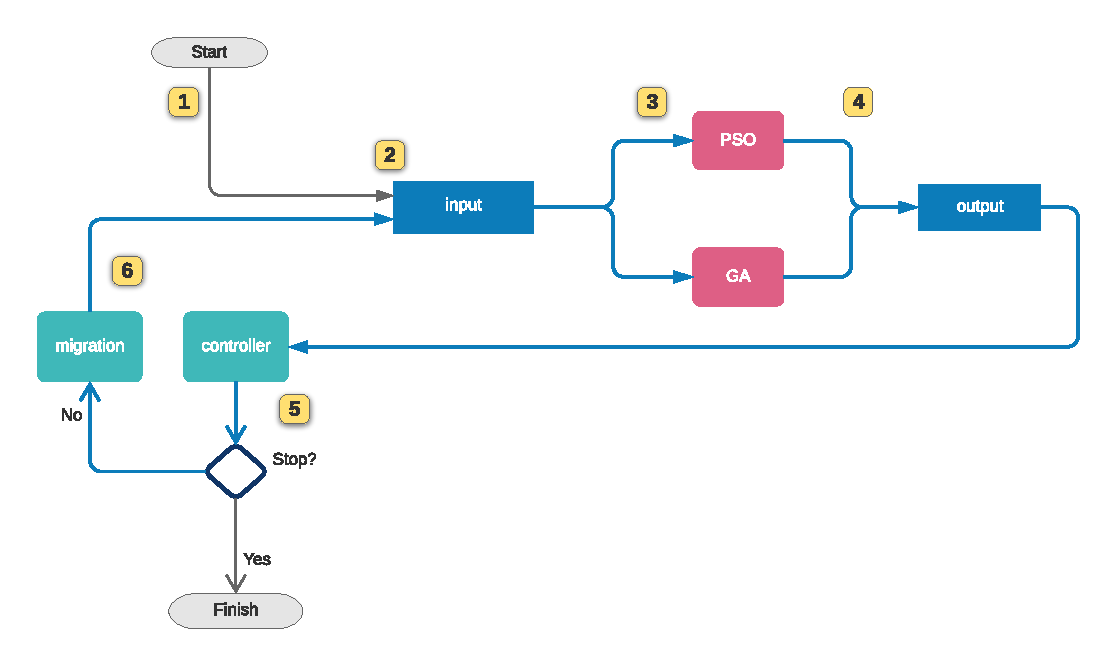
\includegraphics[width=5in]{../images/kafkeo}
\caption{General scheme of the architecture of this method. Please
  refer to text for the explanation of the different numbers.}
\label{fig:kafkeo}
\end{figure*}

As we have mentioned before, when designing efficient multi-population
algorithms, we need to consider additional issues \cite{Ma2019},
including the number and size of populations, how they interact or
communicate between them, and the search strategy and parametrization
of populations. We have considered these requirements and, in this
paper, propose a cloud-native hybrid-algorithm, multi-population
solution. In this model, populations are the primary data structures,
and we package them as messages that are part of a continuous stream
flow from one computing node, that performs a kind of allgorithm, to
the next. To achieve this ``continuous stream,'' everything must
happen asynchronously without. Computing nodes running an algorithm
``wake up'' when they receive a message, with no idle time between the
processing of messages arriving from the stream.

We implemented this streaming functionality by using a message
queue system, we show the architecture in Figure
\ref{fig:kafkeo}. The main components of the architecture are 
producers and consumers of messages. There are two queues, one labeled
\texttt{input}, which mainly holds populations that are going to be
evolved, and the other called \texttt{output} which is where algorithm
nodes send their population messages. In a queue, {\em push}
operations are shown as arrows entering to the left side
and pull or pop operations as arrows leaving from the right
side. The \texttt{controller} process, is responsible for the
migration of individuals from one population to the other, and keeping
track of the iterations of the algorithm. There should be at least one
\texttt{stateless\_function} worker responsible for running an isolated algorithm.
In this case, there are two isolated processes \texttt{PSO} and \texttt{GA},
shown in red. The stream of messages follows the path explained next:

\begin{enumerate}

\item As a first step, a specified number of populations is created. 
At first populations are just data, that includes randomly created individuals.
Each populations has its corresponding metadata section with the algorithm's parameters.
For instance, the parameters for a GA, include the mutation rate, the type of crossover, among others.

\item The setup process pushes each population on to the \texttt{input}
queue, this queue in turn is consumed by all the \texttt{stateless\_functions} executing 
the search algorithms.

\item These functions have the task of executing the optimization algorithm, taking the 
current state of the population to run the algorithm for a specified number of
iterations. When creating a population message, the setup function randomly
selects an optimization algorithm and parameters. These parameters
are part of the population's metadata read by the stateless
functions executing the algorithm. In the current configuration, all
types of algorithms have the same probability of been chosen. % What
                                % happens then with this when
                                % populations are mixed? Which
                                % algorithm is chosen? 
                                % Answered above - M 

\item Once a stateless function finishes the execution of a certain number of
  generations, the resulting population is pushed to 
the \texttt{output} queue; when the computing node is done with a population, it draws another one from the
queue.

\item The \texttt{controller} takes populations from the \texttt{output} queue,
logs the metadata of the current state of each population, and it stops the execution
of the algorithm if an optimal solution has been found or a maximum number of iteration
has been reached.

\item If not, it sends the incoming messages to a ``migration'' function,
  responsible for mixing the populations. This function generates new populations,
  that are again pushed to the \texttt{input} queue closing the loop.
  Although this steps corresponds roughly to the classical
{\em migration}, since it mixes different populations, it is actually
a selection procecure, since it ranks the individuals of the mixed
population according to fitness and selects the best half of them,
eventually generating three new populations. Without this step, there
would be no real parallel algorithm; populations would be sequentially
processed by different algorithms, though.

\end{enumerate}

This message queue pattern is a common component of highly
scalable reactive architectures; one of the reasons for this
scalability is the use of stateless functions. Stateless
functions do not need to read, keep, or modify data outside of the
scope of the method, it will have no side effects reading inputs and
producing an output, mapping input to output as it were. If we
implement population-based optimization algorithms using stateless
functions, then to the system, there is no difference between having
one or many copies of the same function pulling work from the queue
all at the same time. This architecture has been implemented successfully for
developing cloud-native multi-population algorithms, using serverless
functions \cite{garcia2018modern}, and concurrent programming
\cite{guervos2019improving}.
                             % Probably add something about how this
                             % goes beyond the state of the art, by
                             % adding additional diversity- JJ
                             % Should we reference the journal paper
                             % also? - M
% Maybe, anonymously and if there's space for it - JJ

To have a stateless version of a population-based algorithm, we only need to
skip the step of creating a random population. Instead, the function receives
the population as a parameter along with the required parameters. After several
iterations (specified in the parameters), the function returns the current state
of the population, with additional data describing the local execution. This
data is necessary to log the \#FE and current fitness values.

As the controller is pulling population messages from the output
queue, it waits until the message queue contains three valid
populations to trigger an event handled by the
\texttt{population\_mixer} function, which uses as an argument a list
containing the three populations. This design has the advantage of not
needing to keep a buffer in memory or external storage, and following
the reactive paradigm. A possible disadvantage can be that it only
mixes populations that have arrived sequentially to the message queue,
but we could mitigate this with a larger buffer and in fact
populations do not need to arrive to the buffer in the same order they
were created or processed, so this shouldn't, in principle, contribute
to any loss of diversity. The output queue composition depends on two factors:
The number or ratio between each type of algorithm and
the amount of time required to finish the required
number of iterations specified for each population.
For instance, if the implementation of a PSO algorithm
could finish faster than a GA implementation for the
same number of iterations, or if we have more
functions executing a particular algorithm, we will
have more messages from one of the algorithms in the
output queue.

When the \texttt{population\_mixer} unit receives a list of three
populations, let us say [A, B, C], ranking the union of two
populations and generating new ones by merging the best half from
each. Finally, the three generated 
populations back to the \texttt{input} message queue.
We will use this set up to perform a series of experiments destined to
measure the performance of this hybrid algorithm. We will do this next.

% Maybe add an anonymous link to GitHub? - JJ
% Ok, This needs to be a functional link? To see the best option, some things in the 
% actual repo are not anonymous - M
% Nor really. Just the hint of a link - JJ


\section{Experimental setup}
\label{setup}

In this section, we present the experimental setup needed 
to verify if a multi-population algorithm, using asynchronous
heterogeneous populations with a migration procedure, has better performance 
than a single homogeneous algorithm method, needing fewer function evaluations to 
reach a solution. % Maybe say something about the parallel
                            % setup too? - JJ
                            % added the async - Mario

% Use present perfect more than past - JJ
% ok - M
For the experiment, we use five
benchmark separable functions ($f_1 to f_5 $) from the Continuous Noiseless
BBOB testbed, which is part of the Comparing Continuous Optimizers (COCO)
framework \cite{hansen2016coco}. Although there are not many real-world
problems that are entirely separable, we want to focus on these five separable functions
as a primary benchmark for testing the performance of a hybrid multi-population
algorithm. And there is interest in solving such problems using more
general methods \cite{doerr2013evolutionary,swarzberg1994step}. 
% Say why only 5, and these 5 - JJ
% Answered above, short answer: it's a start  - M

These functions are real-parameter, single-objective, and are
usually employed as benchmarks. We have tested with fifteen instances of each
function, each one having a different optimal value. The standard benchmark of
the BBOB testbed % which testbed? % BBOB -M
uses these 15 instances over 2, 3, 5, 10, 20, and
40 dimensions. With the maximum number of function evaluations (\#FEs)
increasing with the dimension (D), using the expression $10^5 \cdot D$ (i.e.
for $D = 2$, \#FEs is $200,000$).
%
% Not that important removing for space - M
%The COCO framework offers several tools to compare the performance of
%algorithms, generating data sets, tables, and reports for an experiment, we have
%compared  using the average required time (aRT). There is a
%repository\footnote{\url{https://coco.gforge.inria.fr/doku.php?id=algorithms-bbob}}
%of more than 200 results for the noiseless BBOB testbed, collected from BBOB
%workshops and special sessions between the years 2009 and 2019.
To test our proposal, we compare the aRT between 
an ensemble of multi-populations,  and single version algorithms using Genetic Algorithms
(GAs) and Particle Swarm Optimization (PSO).

The stateless GA function is implemented using DEAP
\cite{fortin2012deap}, while the PSO algorithm uses EvoloPy
\cite{faris2016evolopy}. These libraries are free software written in
Python, and easily deployable in our framework or in the cloud.  We
show the parameters for each algorithm in Table \ref{tab:GAparams};
these were obtained by following a method proposed by García et al. in
\cite{garcia2017benchmarking:anon} and have been also used in
\cite{GARCIAVALDEZ2021234:anon}. We randomly (within the range shown
in the table) set mutation and crossover probabilities for the GA with
the goal of having more diverse populations and less parameters to
tune. We did not follow the same tactic for PSO, as we choose the same
parameters as those proposed by El-Abd and Kamel in the PSO
implementation for the BBOB benchmark \cite{el2009blackHybrid}. We
have not changed these settings during the experiments, and we have
only provided the population size and number of generations as
parameters.

\begin{table}
  \small
  \caption{ DEAP GA and EvoloPy PSO Parameters }
  \label{tab:GAparams} 
  \centering
  \small
  \begin{tabular}{|l|c||l|c|}
    \hline
    \multicolumn{2}{|c||}{GA} & \multicolumn{2}{c|}{PSO} \\ \hline
    Selection & Tournament size=12 &      $V_{max}$ & 6                  \\ \hline
    Mutation & Gaussian $\mu=0.0$, $\sigma=0.5$, indbp=0.05 & $W_{max}$ & $0.9$     \\ \hline
    Mutation Probability & [0.1,0.3] &   $W_{min}$ & $0.2$                      \\ \hline
    Crossover & Two Point   &       $C_1$ & 2                             \\ \hline
    Crossover Probability  & [0.2,0.6] & $C_2$ & 2  \\ \hline
  \end{tabular}
\end{table}

To run the experiments, we have deployed the Docker application with 8 worker
containers hosting the stateless version of the GA and PSO algorithms described
earlier, and a total of 10 populations. This setup is similar, and in
fact precedes, the one published in \cite{GARCIAVALDEZ2021234:anon}.
\autoref{tab:params:10} shows the parameters we have used (which
also match the ones used in \cite{GARCIAVALDEZ2021234:anon}. The {\em
GA-PSO Ratio} parameter specifies the proportion of populations that
will be processed using the GA algorithm, with $0$ indicating all
populations will run a PSO algorithm, and with $0.5$ the same
proportion of PSO and GA populations, and GA only it is specified with
$1$. We have specified that the experiment will use only the first
five functions. We have used the
standard number of instances in the BBOB benchmark
\cite{hansen2016coco}, 15. The list of
dimensions that we have tested is in the {\em Dimensions} parameter.
Then, we have defined for each dimension: the number of populations,
and for each population, the number of generations and population
size. Finally, we have defined how many complete loops the algorithm
will perform. The product of these parameters gives us a maximum
\#FEs. For example, for $D = 2$, the maximum number of evaluations is
$200,000$, which is equal to $40*50*10*10$ (first column in \autoref{tab:params:10}).

\begin{table}[h!tb]
  \small
  \caption{Parameters used in the experiments, for ten populations and eight workers.
  }
  \label{tab:params:10}
  \vspace{0.25cm}
  \centering
  \small
  \begin{tabular}{|l|c|c|c|c|c|c|}
    \hline
    Dimension        & 2  & 3  & 5  & 10 & 20  & 40  \\ \hline
    Generations      & 40 & 25 & 28 & 50 & 66  & 80  \\ \hline
    Population Size  & 50 & 60 & 60 & 70 & 100 & 125 \\ \hline
    Populations      & 10 & 10 & 10 & 10 & 10  & 10  \\ \hline
    Iterations       & 10 & 20 & 30 & 30 & 30  & 40  \\ \hline
  \end{tabular}
\end{table}

We have deployed the container-based application in a Desktop PC with
AMD Ryzen 9 3900x 12-core processor with 24 threads and 16 GB RAM. We
used Docker version 19.03.3, build a872fc2f86, and {\tt
docker-compose} version 1.21.0, in Ubuntu Linux 18.04, and Python
3.7.5 code. Container images and Docker compose file are available at
(https://hub.docker.com/x/x), and (https://github.com/x/).  The
experiments were performed with COCO \cite{hansen2016coco} version
bbob.v15.03 in python, the plots were produced with version 2.3.2.

\begin{figure*}[h!tb]
    \begin{tabular}
        {c@{\hspace*{-0.00001\textwidth}}
         c@{\hspace*{-0.00001\textwidth}}
         c@{\hspace*{-0.00001\textwidth}}
        }
    GA  &  PSO & GA \& PSO\\   
    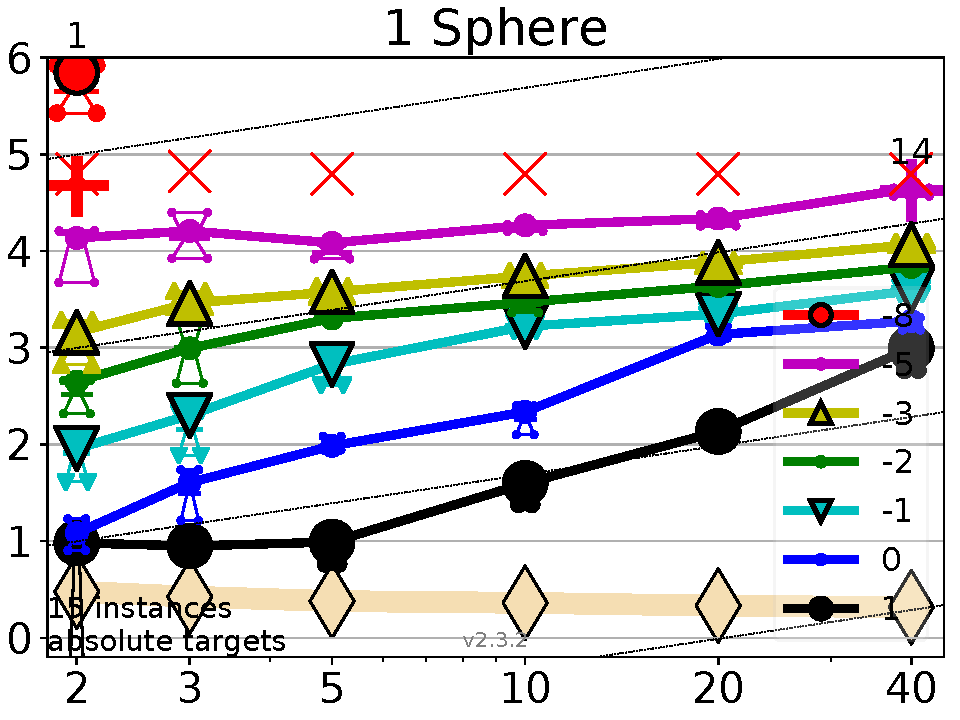
\includegraphics[width=0.28\textwidth]{GAOnly_f001}&
    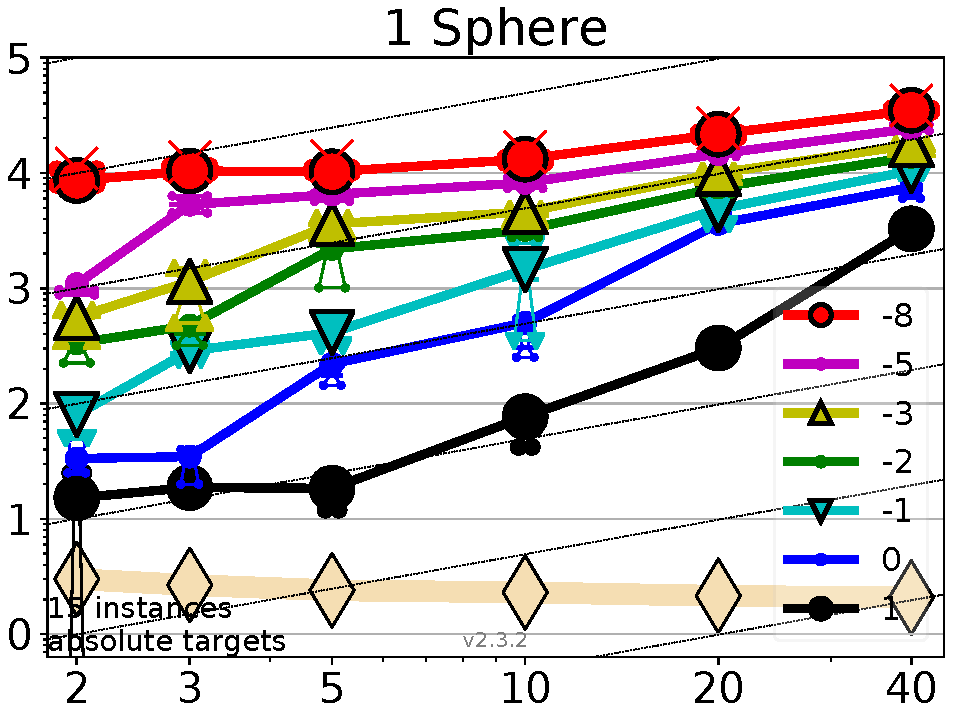
\includegraphics[width=0.28\textwidth]{PSOOnly_f001}&
    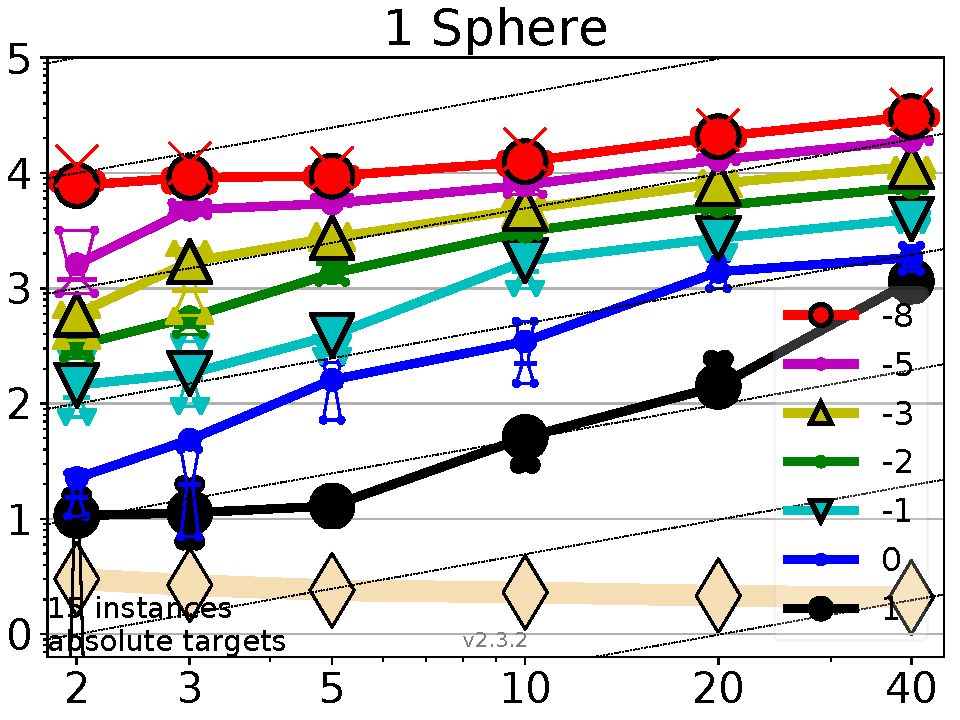
\includegraphics[width=0.28\textwidth]{GAPSO_f001}\\

    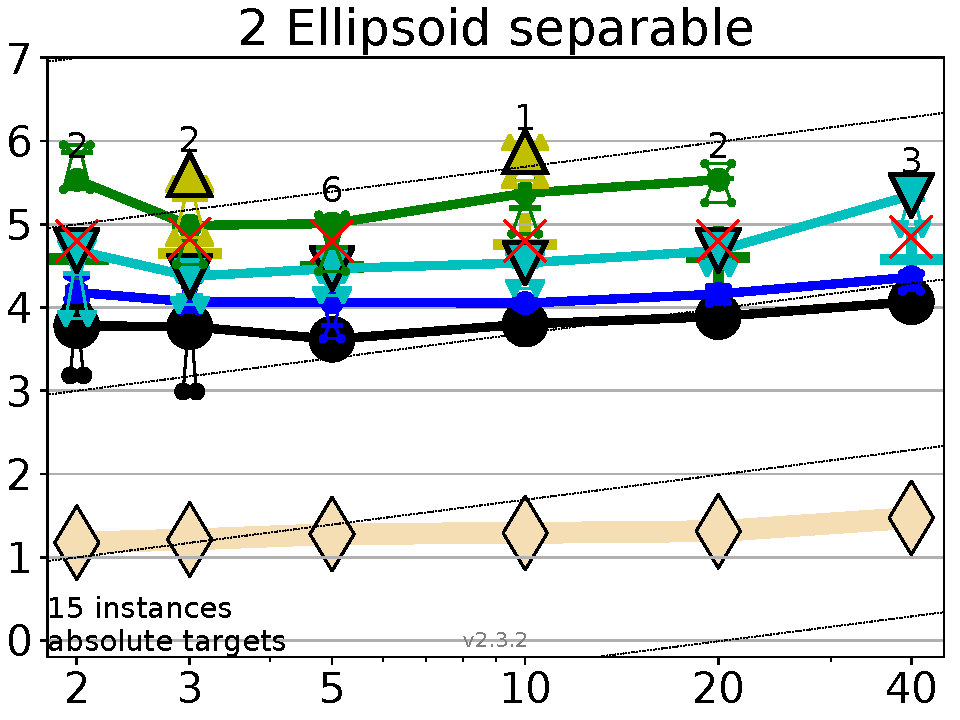
\includegraphics[width=0.28\textwidth]{GAOnly_f002}&
    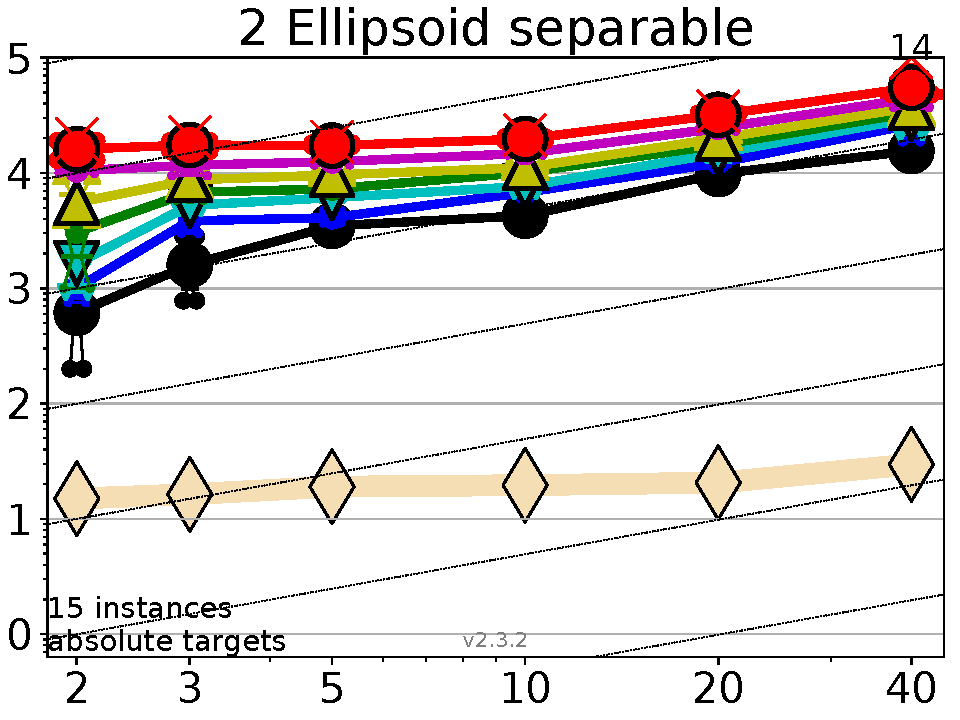
\includegraphics[width=0.28\textwidth]{PSOOnly_f002}&
    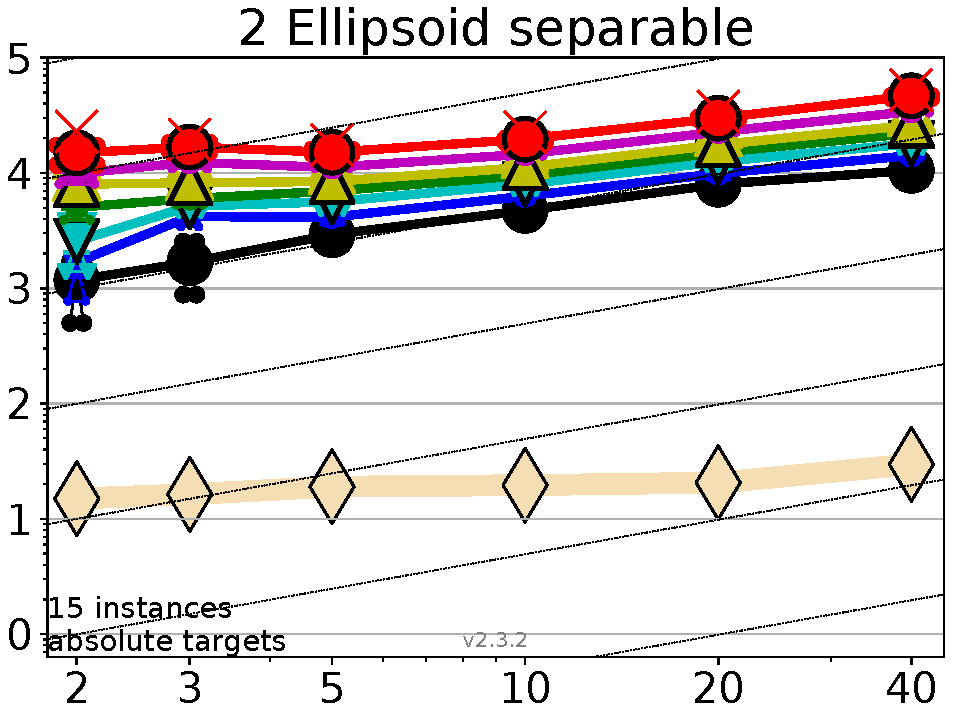
\includegraphics[width=0.28\textwidth]{GAPSO_f002}\\

    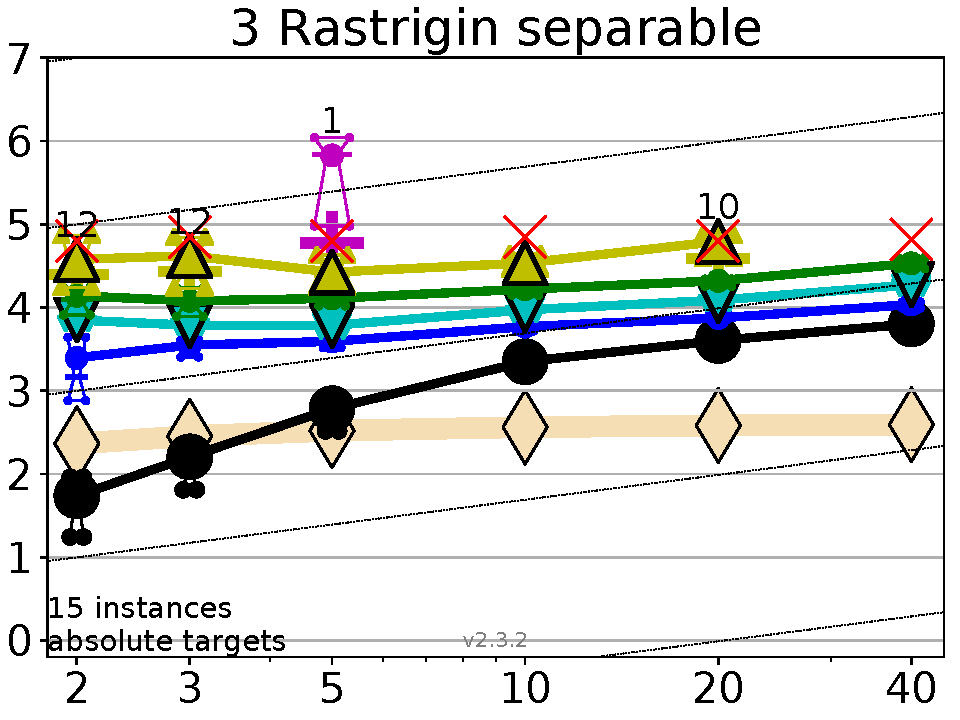
\includegraphics[width=0.28\textwidth]{GAOnly_f003}&
    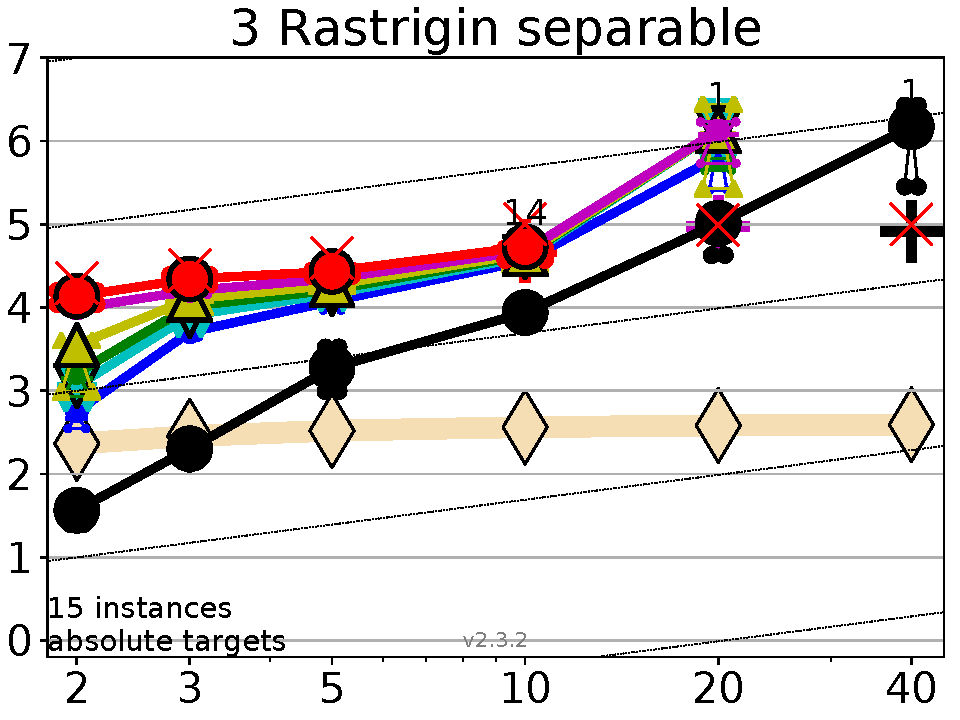
\includegraphics[width=0.28\textwidth]{PSOOnly_f003}&
    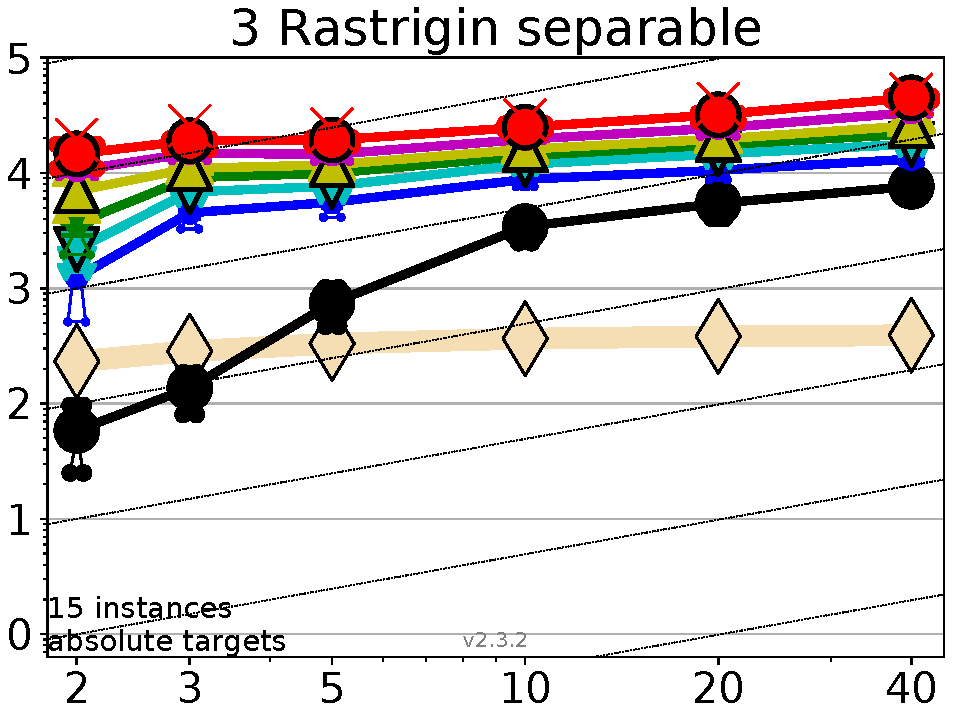
\includegraphics[width=0.28\textwidth]{GAPSO_f003}\\

    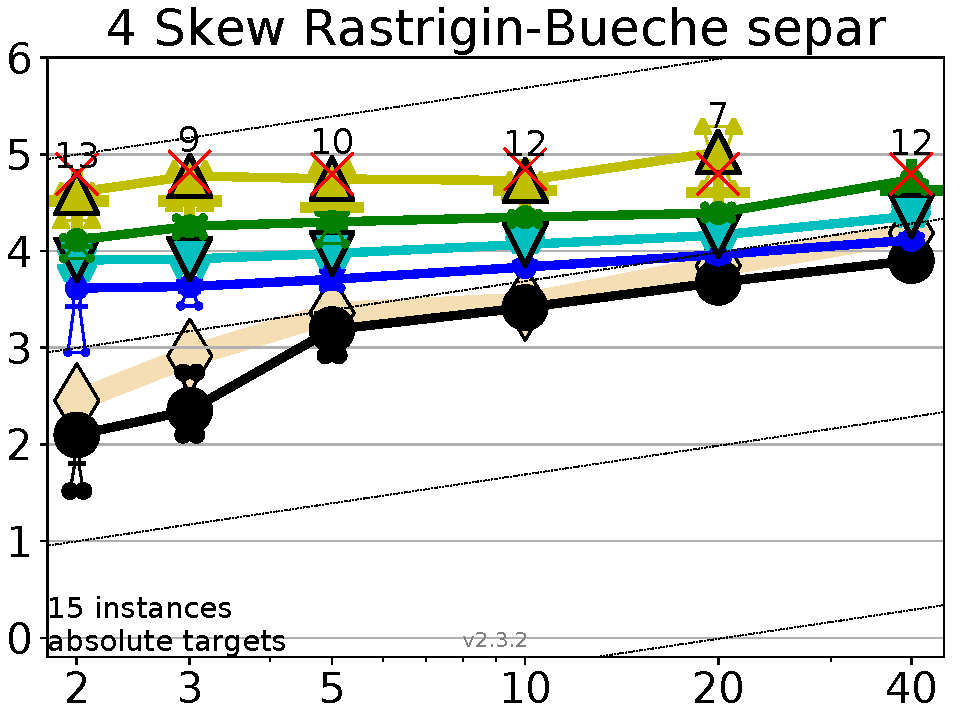
\includegraphics[width=0.28\textwidth]{GAOnly_f004}&
    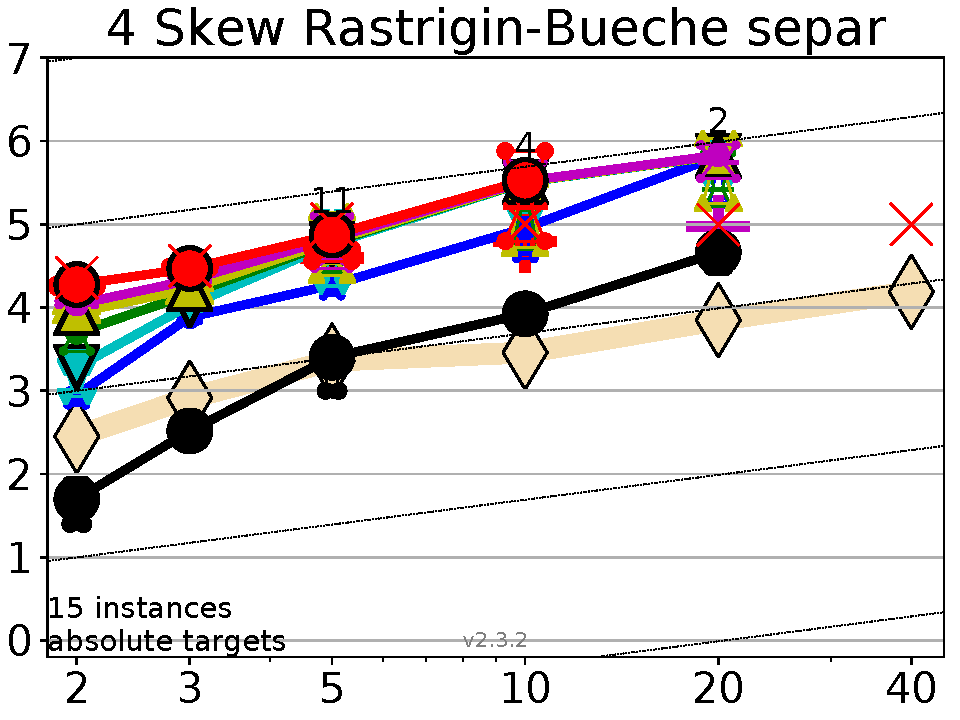
\includegraphics[width=0.28\textwidth]{PSOOnly_f004}&
    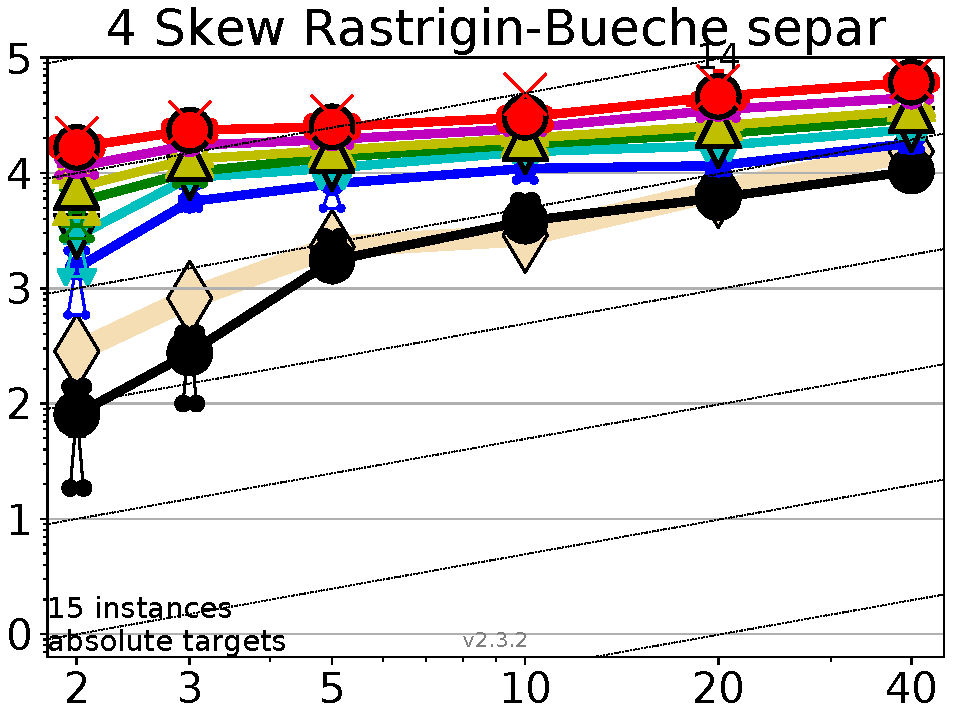
\includegraphics[width=0.28\textwidth]{GAPSO_f004}\\

    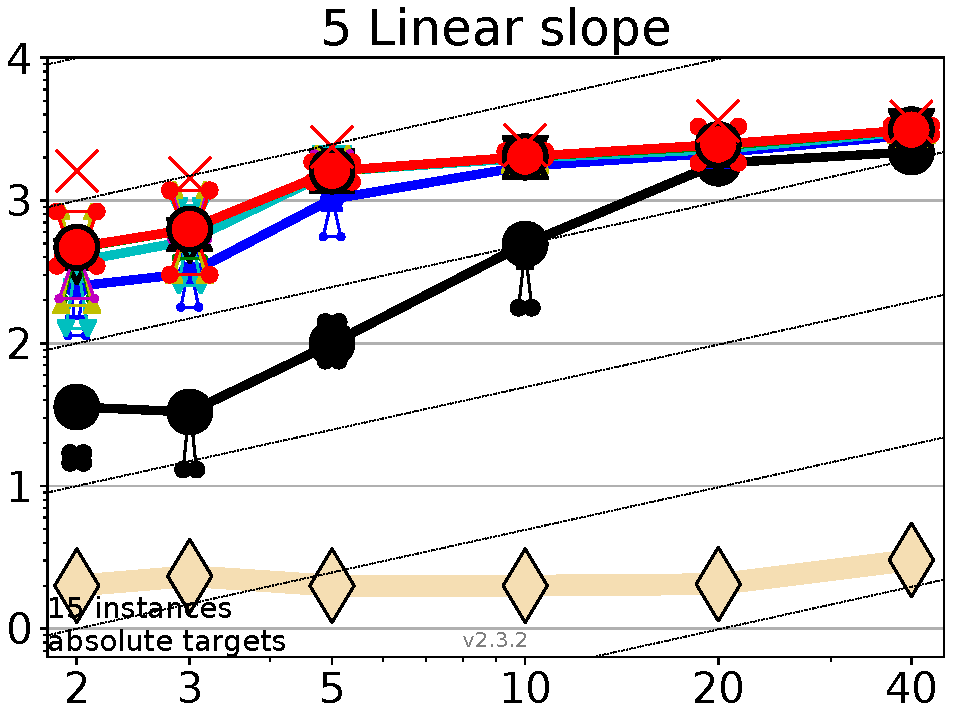
\includegraphics[width=0.28\textwidth]{GAOnly_f005}&
    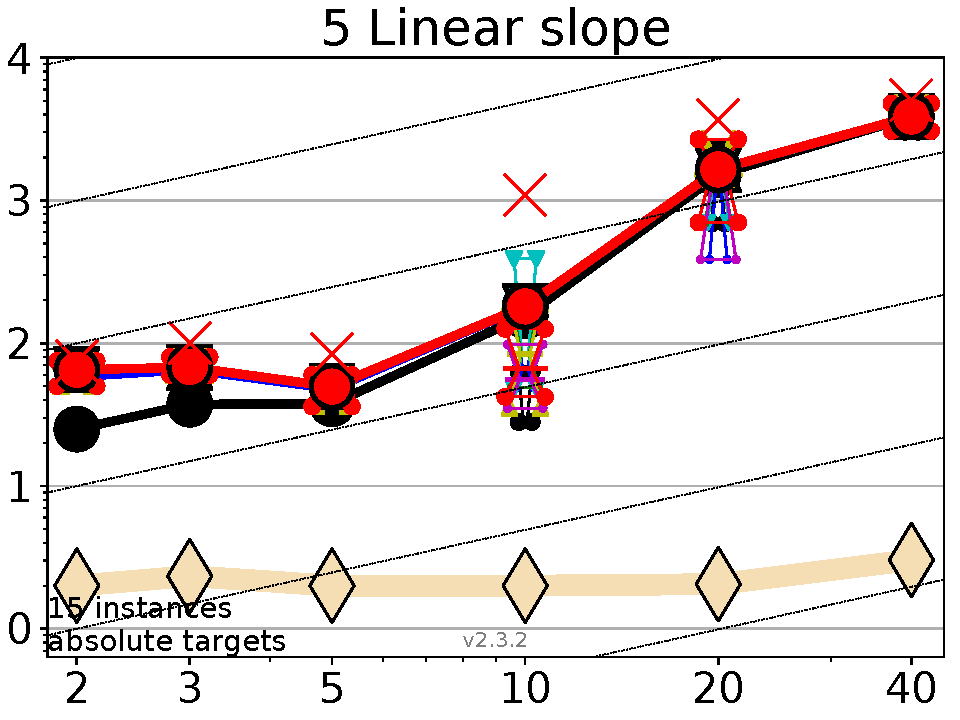
\includegraphics[width=0.28\textwidth]{PSOOnly_f005}&
    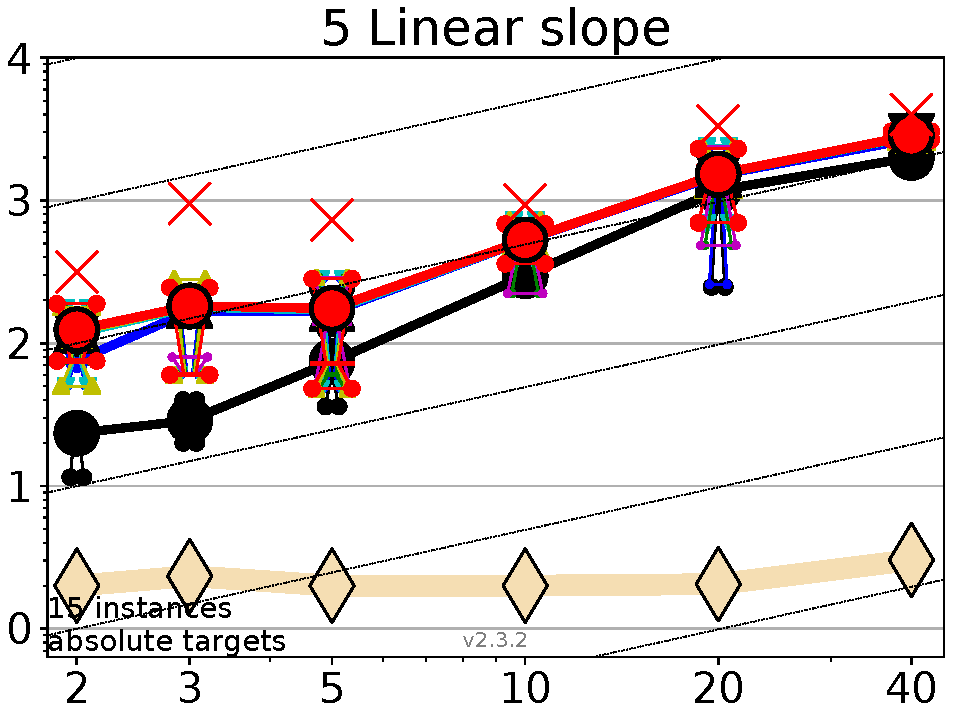
\includegraphics[width=0.28\textwidth]{GAPSO_f005}\\
    \end{tabular}
    \vspace{-3ex}
     \caption{ Running time needed to reach $\Delta f$ ($y$, in log$_{10}$
       scale, divided by dimension) vs. dimension ($x$). Lines:
 average runtime (aRT); ($+$): median runtime of successful runs to reach
 the most difficult target that was reached at least once;
 (\textcolor{red}{$\times$}): maximum number of evaluations in any trial. Notched boxes:
 interquartile range with median of simulated runs. Please note that
 $y$ in the same row, generated automatically by COCO, can be different.}
\label{fig:bbob}
\end{figure*}


\begin{figure*}[h!tb]
  \begin{tabular}
      {c@{\hspace*{-0.00001\textwidth}}
       c@{\hspace*{-0.00001\textwidth}}
       c@{\hspace*{-0.00001\textwidth}}
      }
  10D &  20D & 40D\\   
  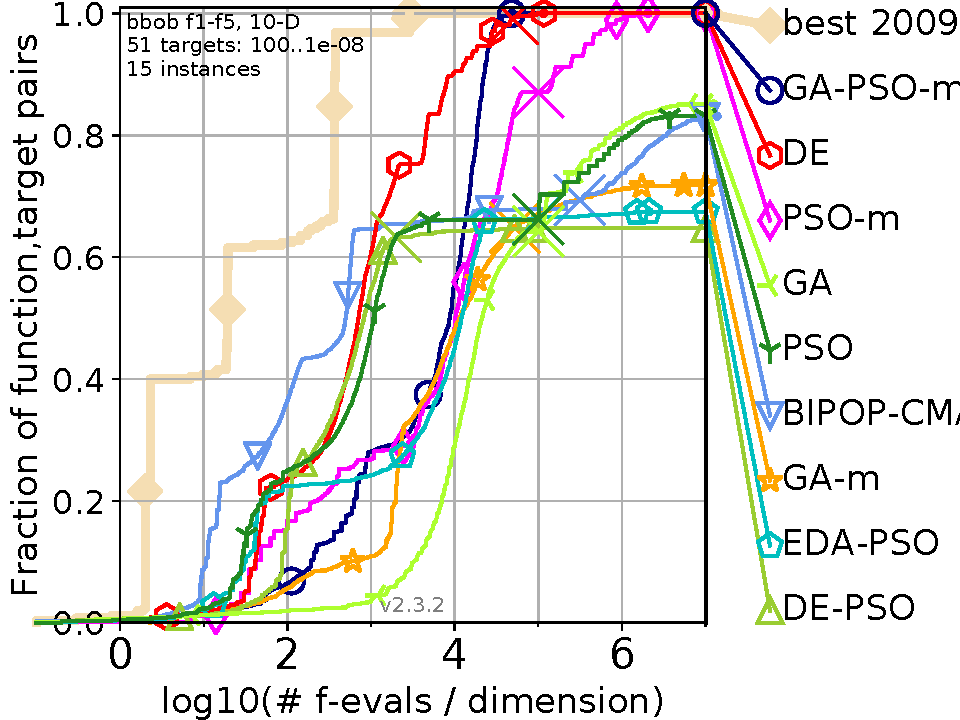
\includegraphics[width=0.30\textwidth]{pprldmany_10D_separ}&
  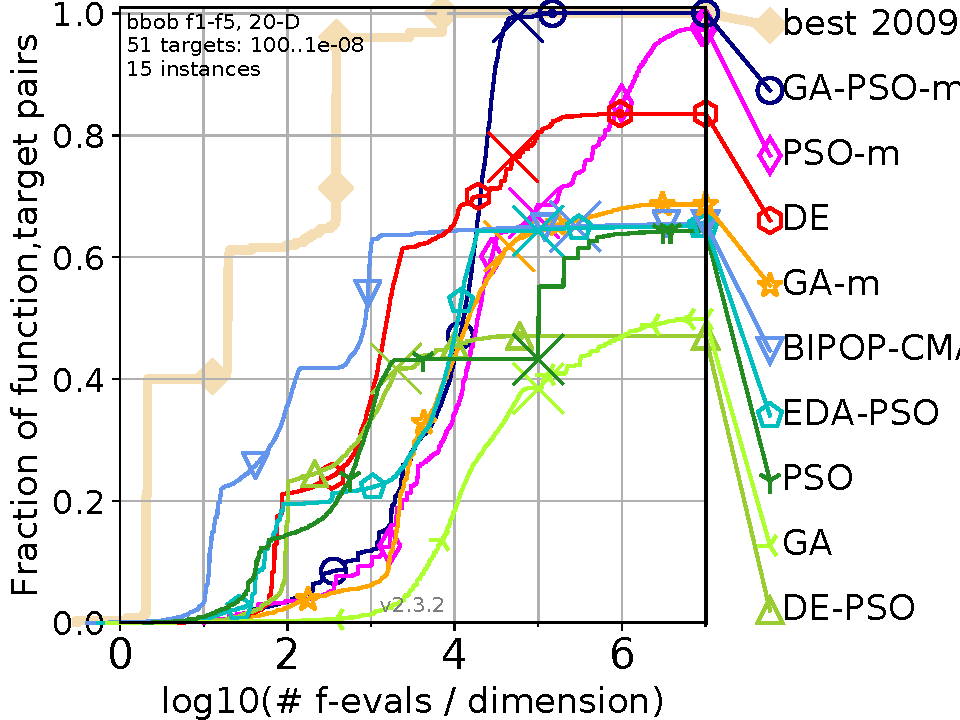
\includegraphics[width=0.30\textwidth]{pprldmany_20D_separ}&
  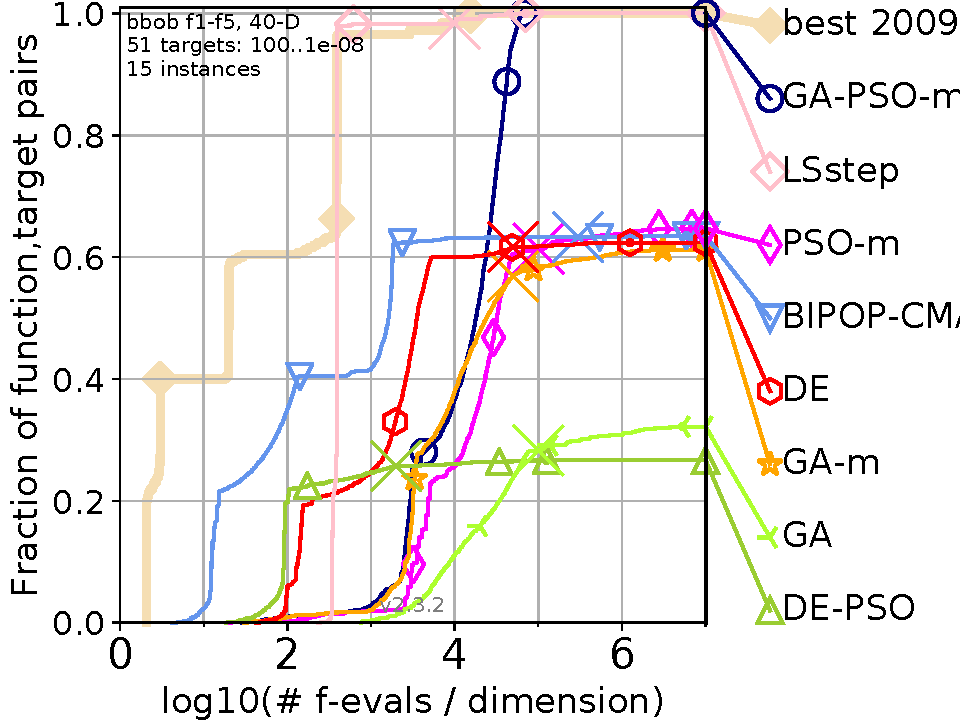
\includegraphics[width=0.30\textwidth]{pprldmany_40D_separ}\\

\end{tabular} \vspace{-3ex} \caption{Bootstrapped empirical cumulative
distribution of the number of objective function evaluations divided by
dimension (FEvals/DIM) for the functions used in this paper. } \label{fig:bbob2} 
\end{figure*}
%
\section{Results}
\label{results}

The results are shown in Figure \ref{fig:bbob}, where we can see how
the runtime scales with dimension, for reaching certain target values $\Delta f$;
% Please check that this is true - JJ
% One compares between our own multi-populations the other against the rest 
% and only for the hardest target 10^(-8) - Mario
% The last one, shows #FE vs Percentege of $10^{-8}$ targets reached
% Our GA-PSO reaches almost all targets, but takes more #FE than others
% That is why appears on top. It reaches but takes more evals on average.
% So please fix that... - JJ
% ping here - JJ
% TO DO - M
% Was fixed in another commit - M
line colors indicate the average runtime for targets reached
at least one time. A red circle without a number on top indicates the algorithm
has reached the most difficult target $10^{-8}$ on all instances for that dimension;
if it has a number, this indicates how many times the target was reached.
Values of targets $\Delta f = 10^{k}$ with $k$ colors are
given in the legend of the first function, $k$ values are $[-8,-5,-3,-2,-1,0,1]$. 
Each column presents the results for GA, PSO, and GA\&PSO methods.
The GA algorithm (on the left column) has more difficulty even to reach the
$10^{-5}$ target in functions ($f_1-f_4$) for all dimensions, and has the worst
performance in 20 and 40 dimensions. It performs better on function five $f_5$
where it reaches the $10^{-8}$ target on all dimensions, but it has the highest runtime on lower
dimensions. 

            % Maybe some comments on why these 5 functions and what
            % makes f5 special? - JJ
            % This was mentioned earlier, F5 I think is more deceptive, but I'm not sure will check that - M   
            % TO DO
The multi-population PSO on the other hand (shown in the middle),
has better performance; reaching all targets for functions $f_1$ and $f_2$ but 
it has a higher runtime in most cases when compared against the multi-strategy method. 
PSO is not able to reach the $10^{-8}$ target on functions $f_3$ and $f_4$ for higher dimensions; 
but it has the best overall runtime for the lower dimensions of $f_5$.

\begin{figure}[h!tb]
  \begin{tabular}
      {c@{\hspace*{-0.00001\textwidth}}
      % c@{\hspace*{-0.00001\textwidth}}
      }
     
  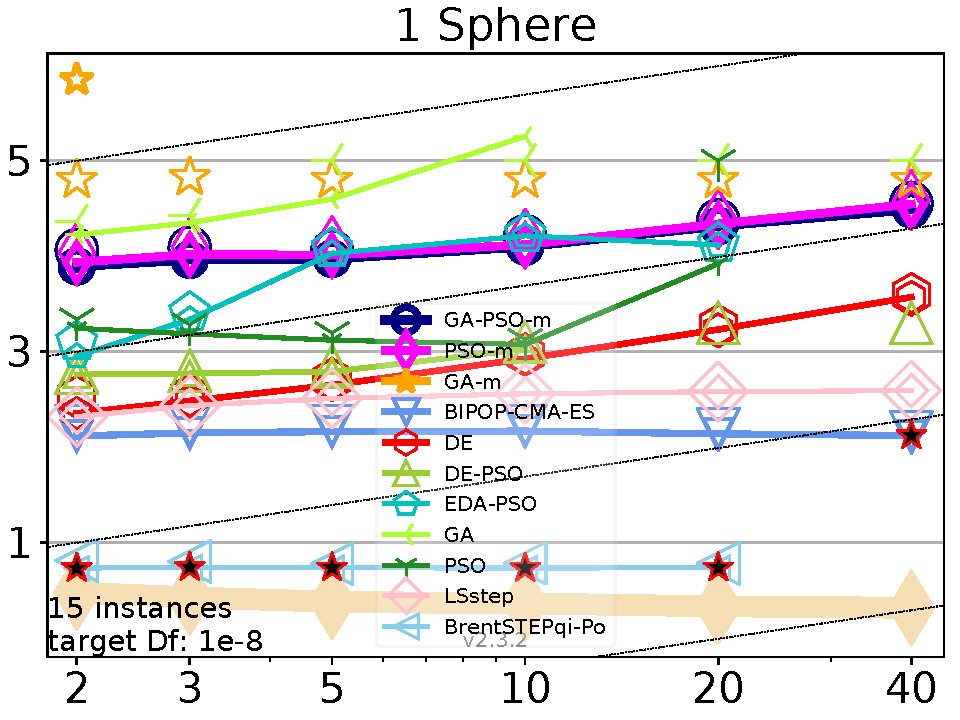
\includegraphics[width=0.30\textwidth]{ppfigs_f001}
  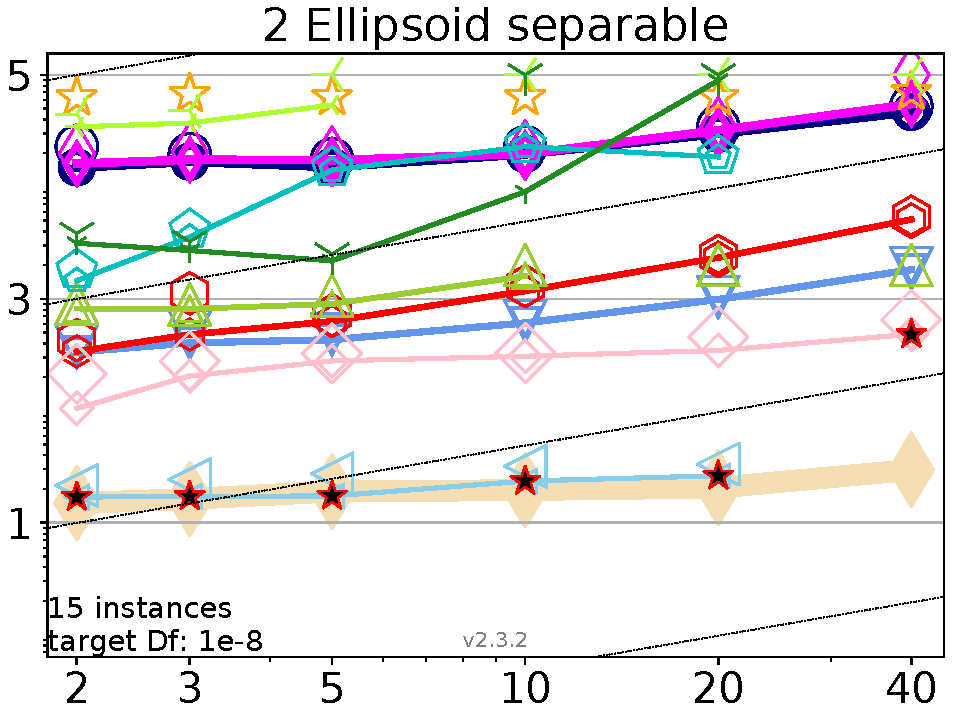
\includegraphics[width=0.30\textwidth]{ppfigs_f002}

  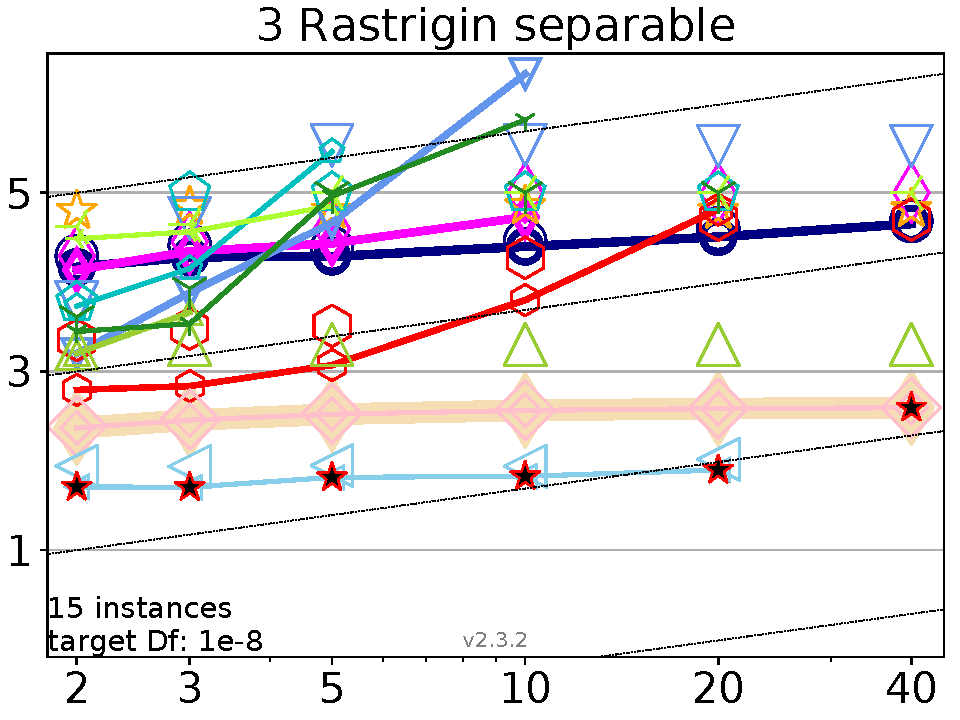
\includegraphics[width=0.30\textwidth]{ppfigs_f003}\\
  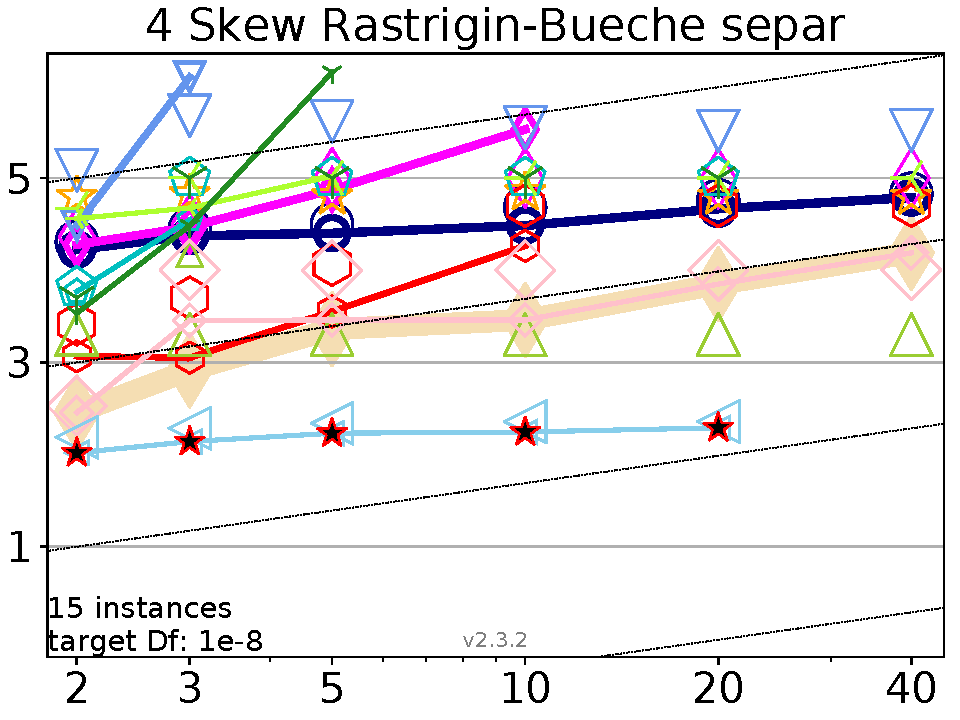
\includegraphics[width=0.30\textwidth]{ppfigs_f004}
  
  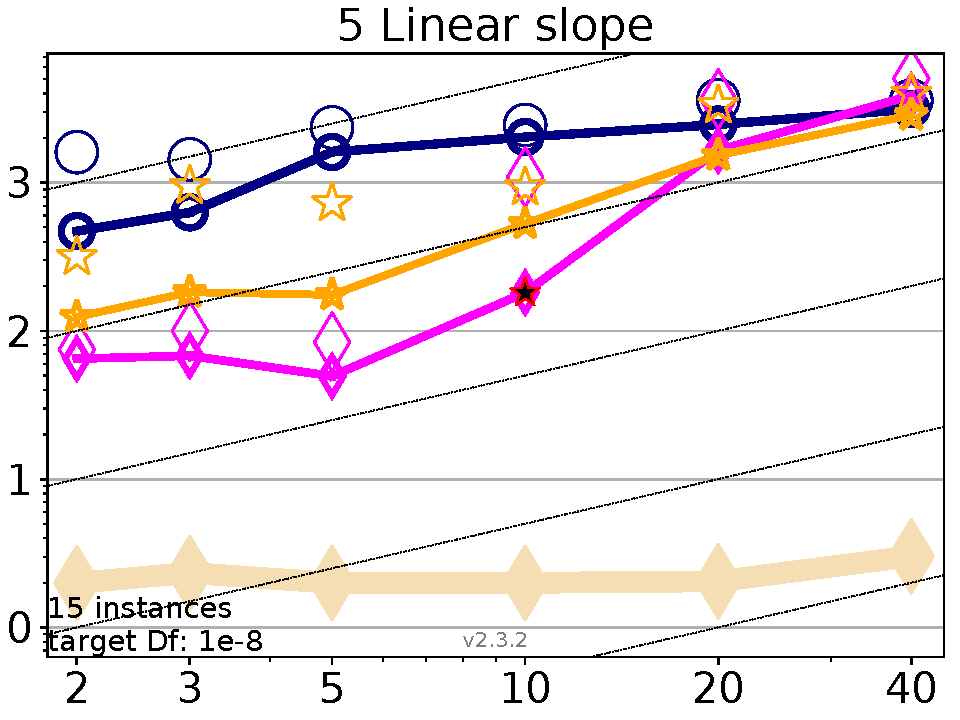
\includegraphics[width=0.30\textwidth]{ppfigs_f005}
  \end{tabular}
  \vspace{-3ex}
   \caption{Average running time (in \#FEs as $log_{10}$ value)
     normalized by dimension for target function value $10^{-8}$ ($y$)
     per dimension ($x$). Black stars mark significantly better
     results.
    Legend: {\color{NavyBlue}$\circ$}:GA-PSO-m, 
    {\color{Magenta}$\diamondsuit$}:PSO-m, 
    {\color{Orange}$\star$}:GA-m, 
    {\color{CornflowerBlue}$\triangledown$}:BIPOP-CMA-ES,
    {\color{red}$\varhexagon$}:DE, 
    {\color{YellowGreen}$\triangle$}:DE-PSO, 
    {\color{cyan}$\pentagon$}:EDA-PSO, 
    {\color{GreenYellow}$\rightY$}:GA, 
    {\color{ForestGreen}$\downY$}:PSO, 
    {\color{Lavender}$\Diamond$}:LSstep, 
    {\color{SkyBlue}$\triangleleft$}:BrentSTEP
    } 
  \label{fig:avg}
\end{figure}
%
Finally, the proposed PSO\&GA multi-strategy method reaches the most difficult $10^{-8}$ target
on all functions ($f_1-f_5$) scaling well to higher dimensions, even
on $f_3$ and $f_4$ (charts on the last row), which are usually
considered difficult functions \cite{hansen2010comparing}.  % Maybe a reference for this? - JJ
% I will add the paper of BBOB results showing less algorithms finding the solution.
% Reference added - M
These results are also competitive when compared against other GA and PSO
implementations of past BBOB workshops. Figure \ref{fig:avg} shows
how the runtime scales with dimension to reach the most difficult target
for $\Delta f = 10^{-8}$ for each function.
We chose two types of representative algorithms, first, Evolutionary 
an Swarm based and  not population-based. We chose a simple binary GA algorithm of Nicolau \cite{nicolau2009application},
the PSO algorithm by El-Abd and Kamel \cite{el2009blackHybrid}, an EDA and PSO
hybrid \cite{el2009blackHybrid}, 
Differential Evolution (DE) with adaptive encoding \cite{povsik2012benchmarking}
by {Po{\v{s}}{\'\i}k and Klem{\v{s}},
the hybrid DE-PSO by Garc{\'\i}a-Nieto et
al. \cite{garcia2009noiseless},
and the BIPOP-CMA-ES algorithm \cite{hansen2009benchmarking} by Hansen, this last algorithm has the
best overall ($f_1-f_2$) performance on the BBOB-2009 benchmark,
as it  could solve 23, 22 and 20 functions out of 24 in dimensions 10, 20 and
40, respectively.  The algorith uses two interlaced restart strategies, 
one with an increasing population size and one with varying small population sizes using
a covariance matrix adaptation evolution strategy (CMA-ES).
We also compare with two methods that are not population-based, but univariate
solvers generalized for the optimization of separable functions, the
line-search algorithm LSStep by Po{\v{s}}{\'\i}k \cite{povsik2009bbob}, and the Hybrid Brent-STEP by
Po{\v{s}}{\'\i}k and Baudi{\v{s}} \cite{povsik2015dimension}. The performance for the Brent-STEP algorithm
is the best for this group of functions, finding all targets with less FEs.

We can see that the number of evaluations of {\sf GA-PSO-m} tends to be higher
in most cases, but on the other hand, it could solve all functions
while others could not. This fact is in accordance with our hypothesis
that a having a combination of methods, gives as a result an 
exploration that keeps diversity in balance with exploitation.
It can take more evaluations, but it explores other areas of the search space, avoiding 
local minima in more cases.
                        % We should refer back to our hypothesis of
                        % better exploration of the search space here
                        % - JJ
                        % done - M
As expected, the BIPOP-CMA-ES algorithm has the best running time on functions
$f_1$, $f_2$ and $f_5$ and reaches three targets at search dimensions 20 and 40.
It is worth to notice the performance of the DE algorithm, having the best
running time on lower dimensions of  $f_3$ and $f_4$.
Figure \ref{fig:bbob2} highlights the performance of our proposal in search
space of dimensions 10, 20, and 40. The figure shows the fraction of
functions-target pairs by the number of FEs. In this case, an algorithm that
requires less FEs to reach all targets will have more area under the curve. For
higher dimensions, the GA-PSO multi-population gives competitive results by
reaching all targets within budget. The Brent-STEP algorithm did not provide
results for 40D.

\section{Conclusions, discussion and future lines of work}
\label{conclusions}

A common element of different population based metaheuristics, namely,
the population itself, has made the application of different
algorithms relatively easy by decoupling the algorithms from the
population. In \cite{GARCIAVALDEZ2021234:anon} we showed how this
could be used in a cloud native framework; this paper scales back the
functionality showing a more basic mixed-algorithm, stateless and
concurrent implementation that combines off-the-shelf open source
libraries to create a higher level optimization framework that can be
easily deployed locally or on the cloud. The fact that populations and evolution (or any other kind of
change) are totally decoupled and the processing of every population
is stateless enables the creation create a mixture of processing algorithms that work
asynchronously (and possibly concurrently) and in a way that's totally
independent of each other. More methods can be added to the mix by simply
adding another stateless function that listens to the population queue
and writes back to it.


% A paragraph trying to explain results, looking at the results for
% different functions. Why does it work better? Does it really
% increase diversity? - JJ
% We did not actually tested diversity, will added as a future work - M
% added below - M

We have tested this combination of algorithms on the BBOB benchmark
functions, obtaining results that are better than those obtained by
any of them separated. This confirms results obtained by previous
authors in hybrid algorithms, except that, in this case, the architecture is different and
there are improvements all across the tested functions; besides,
results are better than results that have been published for other
algorithms, including a hybrid one, making the hybrid PSO/GA a firm
contender in the function optimization arena.
It is interesting to note that this is done despite mixing both
algorithms in a totally random way, so that it's really impossible to
know whether an individual population will be processed by a GA or
PSO, or how many cycles of each has undergone. The migration process,
however, guarantees a mixing of results and is probably the key to the
ultimate success of the algorithm proposed here.

As future lines of work, we will try to add different
population-based, data-compatible algorithms to the mix, to see what
kind of results they obtain and what could possible be the best
possible mix. An extensive study on the real effects of the mix of
algorithms should also be performed, with a theoretical basis if possible, using the
size of the basins of attractions, for instance, or how different
algorithms move along the fitness landscape. We can also measure how
diversity is maintained by the combination of methods and random parameters,
and propose new ways to adapt this diversity to the state of the search.

\section*{Acknowledgments}
The authors would also like to thank the anonymous referees for their
helpful suggestions and corrections. 
Supported by the so and so.


\bibliographystyle{splncs04}
\bibliography{multipopulation,hybrid} 

\end{document}
